\documentclass[12pt]{scrartcl}
% LaTeX Template für Abgaben an der Universität Stuttgart
% Autor: Sandro Speth
% Bei Fragen: Sandro.Speth@iste.uni-stuttgart.de
%-----------------------------------------------------------
% Modul fuer verwendete Pakete.
% Neue Pakete einfach einfuegen mit dem \usepackage Befehl:
% \usepackage[options]{packagename}
\usepackage[utf8]{inputenc}
\usepackage[T1]{fontenc}
\usepackage[ngerman]{babel}
\usepackage{lmodern}
\usepackage{graphicx}
\usepackage[pdftex,hyperref,dvipsnames]{xcolor}
\usepackage{listings}
\usepackage[a4paper,lmargin={2cm},rmargin={2cm},tmargin={3.5cm},bmargin = {2.5cm},headheight = {4cm}]{geometry}
\usepackage{amsmath,amssymb,amstext,amsthm}
\usepackage[lined,algonl,boxed]{algorithm2e}
% alternative zu algorithm2e:
%\usepackage[]{algorithm} %counter mit chapter
%\usepackage{algpseudocode}
% \usepackage{tikz}
\usepackage{hyperref}
\usepackage{url}
\usepackage[inline]{enumitem} % Ermöglicht ändern der enum Item Zahlen
\usepackage[headsepline]{scrlayer-scrpage} 
\pagestyle{scrheadings} 
% LaTeX Template für Abgaben an der Universität Stuttgart
% Autor: Sandro Speth
% Bei Fragen: Sandro.Speth@iste.uni-stuttgart.de
%-----------------------------------------------------------
% Modul beinhaltet Befehl fuer Aufgabennummerierung,
% sowie die Header Informationen.

% Überschreibt enumerate Befehl, sodass 1. Ebene Items mit
\renewcommand{\theenumi}{(\alph{enumi})}
% (a), (b), etc. nummeriert werden.
\renewcommand{\labelenumi}{\text{\theenumi}}

% Counter für das Blatt und die Aufgabennummer.
% Ersetze die Nummer des Übungsblattes und die Nummer der Aufgabe
% den Anforderungen entsprechend.
% Gesetz werden die counter in der hauptdatei, damit siese hier nicht jedes mal verändert werden muss
% Beachte:
% \setcounter{countername}{number}: Legt den Wert des Counters fest
% \stepcounter{countername}: Erhöht den Wert des Counters um 1.
\newcounter{sheetnr}
\newcounter{exnum}

% Befehl für die Aufgabentitel
\newcommand{\exercise}[1]{\section*{Aufgabe \theexnum\stepcounter{exnum}: #1}} % Befehl für Aufgabentitel

% Formatierung der Kopfzeile
% \ohead: Setzt rechten Teil der Kopfzeile mit
% Namen und Matrikelnummern aller Bearbeiter
\ohead{Max Mustermann (1234567)\\
Klaus Kleber (1234568)\\
Melanie Marshmallow (1234569)}
% \chead{} kann mittleren Kopfzeilen Teil sezten
% \ihead: Setzt linken Teil der Kopfzeile mit
% Modulnamen, Semester und Übungsblattnummer
\ihead{Datenstrukturen \& Algorithmen\\
Sommersemester 2020\\
Übungsblatt \thesheetnr}

\setcounter{sheetnr}{2} % Nummer des Übungsblattes
\setcounter{exnum}{1} % Nummer der Aufgabe

% Beginn des eigentlichen Dokuments

\begin{document}

% Aufgabe 1
\exercise{Verständnis}
\begin{enumerate}
  \item Die folgenden Funktionen in das gemeinsames Koordinatenssystem
  \begin{figure}[!h]
    \centering
      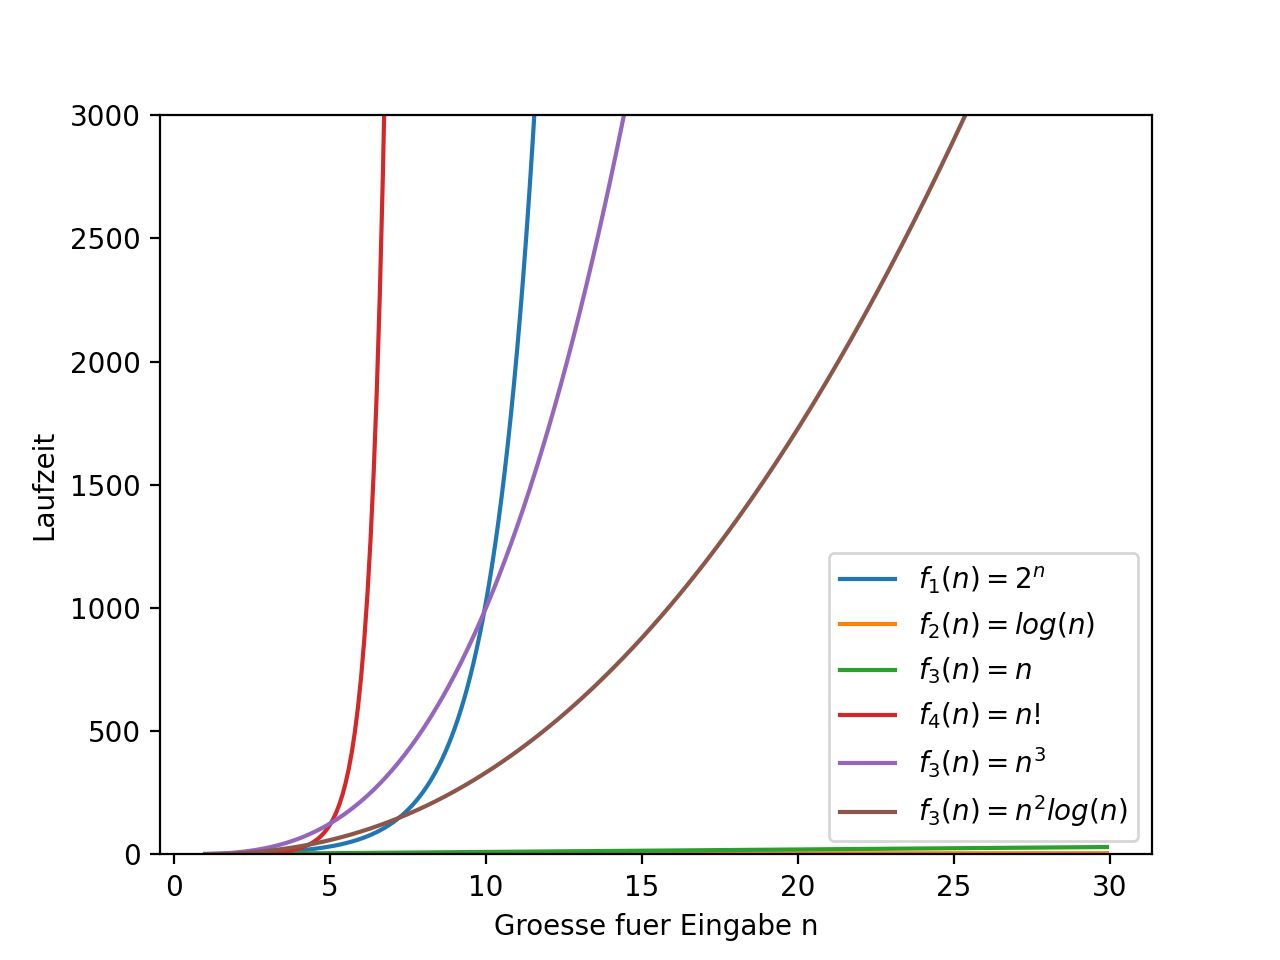
\includegraphics[width=0.5\textwidth]{overview.png}
    \caption{Alle 6 Funktionen in einer Abbildung}
  \end{figure}
  \begin{figure}[!h]
    \centering
      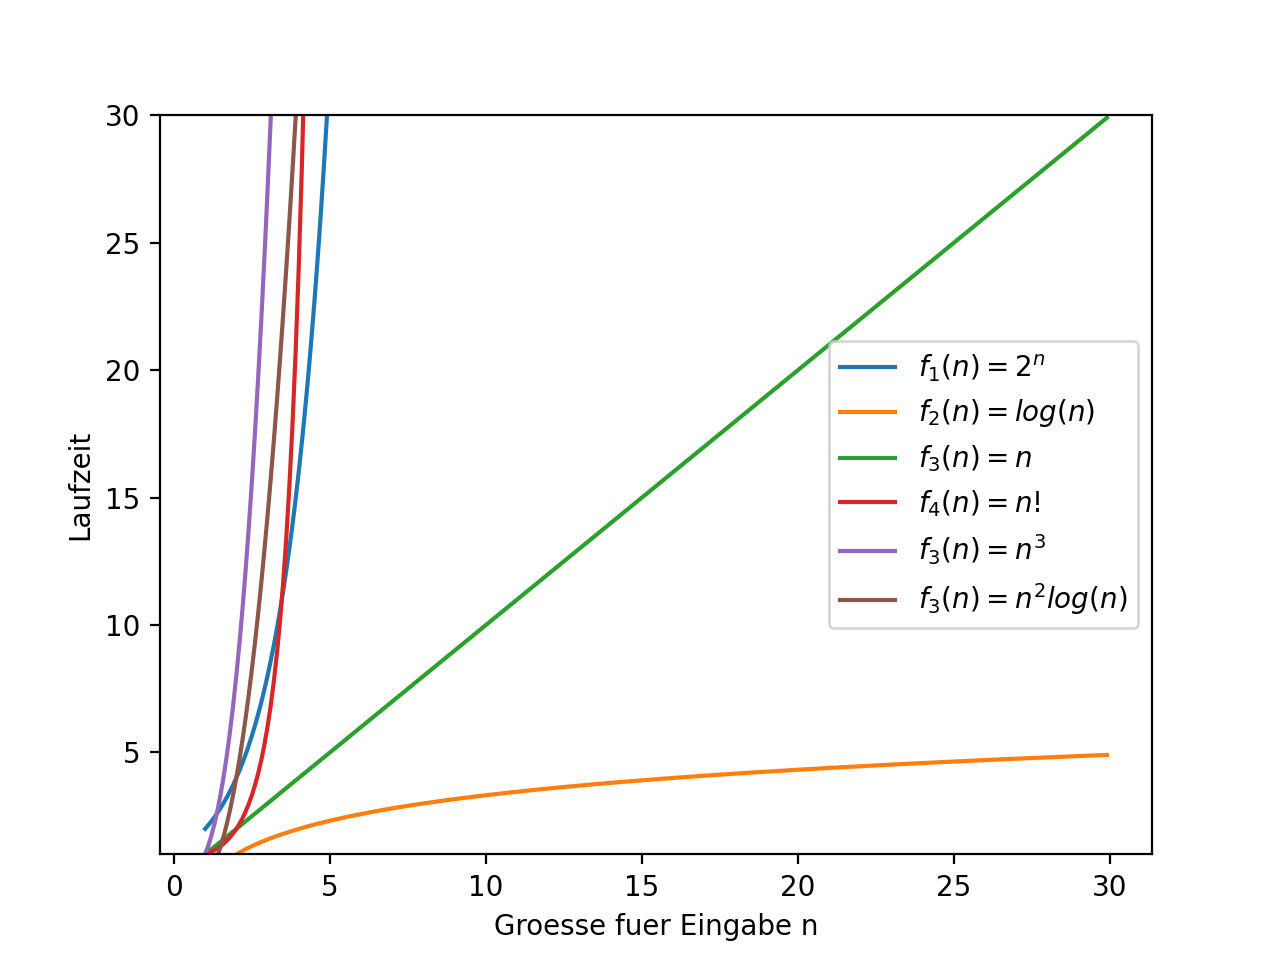
\includegraphics[width=0.5\textwidth]{small_y.png}
    \caption{Nur y-Wert zwischen 0-30 betrachtet wird}
  \end{figure}
  \begin{figure}[!h]
    \centering
      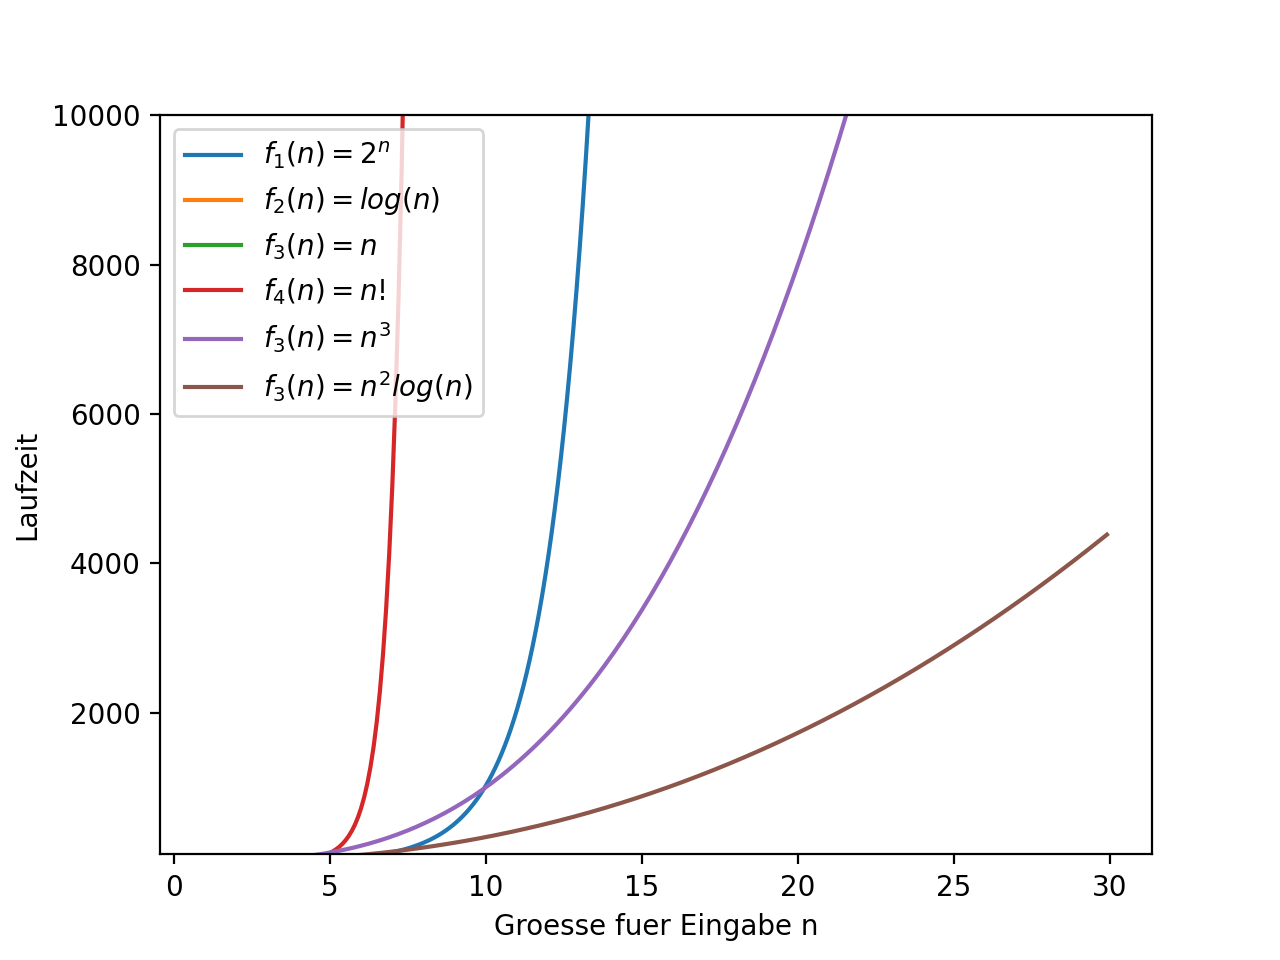
\includegraphics[width=0.5\textwidth]{big_y.png}
    \caption{Größer y-Wert betrachtet wird}
  \end{figure}
  \item $\mathcal{O}(n!) > \mathcal{O}(2^n) > \mathcal{O}(n^3) > \mathcal{O}(n^2log(n)) > \mathcal{O}(n) > \mathcal{O}(log(n))$
  \begin{center}
    \begin{tabular}{ |c|c|c| } 
     \hline
     $f_1(n) = 2^n$ & $\mathcal{O}(2^n)$ & exponenziell \\ 
     $f_2(n) = log(n)$ & $\mathcal{O}(log(n))$ & logarithmisch \\ 
     $f_3(n) = n$ & $\mathcal{O}(n)$ & linear \\ 
     $f_4(n) = n!$ & $\mathcal{O}(n!)$ & faktoriell \\ 
     $f_5(n) = n^3$ & $\mathcal{O}(n^3)$ & polynomiell \\ 
     $f_6(n) = n^2log(n)$ & $\mathcal{O}(n^2log(n))$ & logquadratisch \\ 
     \hline
    \end{tabular}
    \end{center}
\end{enumerate}

% Aufgabe 2
\exercise{Asymptotische Komplexität}
\begin{enumerate}
  \item alg1\\
    for-Schleife i: $\mathcal{O}(n)$\\
    for-Schleife j: $\mathcal{O}(n)$\\
    for-Schleife k: $\mathcal{O}(n)$\\
    Insgesamt: $\mathcal{O}(n)*\mathcal{O}(n)*\mathcal{O}(n) = \mathcal{O}(n^3)$
    \item alg2\\
    while-Schleife: $\mathcal{O}(log{}n)$\\
    for-Schleife i: $\mathcal{O}(n)$\\
    for-Schleife j: $\mathcal{O}(n)$\\
    Insgesamt: $\mathcal{O}(log(n)) + \mathcal{O}(n)*\mathcal{O}(n) = \mathcal{O}(n^2)$
    \item alg3\\
    die erste for-Schleife i: $\mathcal{O}(n)$\\
    die zweite for-Schleife i: $\mathcal{O}(n)$\\
    Insgesamt: $\mathcal{O}(n) + \mathcal{O}(n) = \mathcal{O}(n)$
    \item alg4\\
    $alg4(n) = 2alg4(n-1) = 4alg4(n-2) = ... = 2^{(n-1)}alg2(1)$\\
    Insgesamt: $\mathcal{O}(2^n)$
    \item alg5\\
    if-else: $\mathcal{O}(1)$\\
    for-Schleife i: $\mathcal{O}(n)$\\
    Für alg(n), if-else und for-Schleife werden n mal aufgerufen.\\
    Insgesamt: $\mathcal{O}(n^2)$
    \item alg6\\
    for-Schleife i: $\mathcal{O}(n)$\\
    for-Schleife j: $\mathcal{O}(log(n))$\\
    for-Schleife k: $\mathcal{O}(1)$\\
    Insgesamt: $\mathcal{O}(n)*(\mathcal{O}(log(n)) + \mathcal{O}(1)) = \mathcal{O}(nlog(n))$
\end{enumerate}

\end{document}
